\documentclass[12pt]{article}

\usepackage{sbc-template}

\usepackage{graphicx,url}

%\usepackage[brazil]{babel}   
\usepackage[latin1]{inputenc}  

     
\sloppy

\title{Using Agents \& Artifacts to Access the Semantic Web  \\A Recommender System Case Study }

\author{J�ssica Pauli de C. Bonson\inst{1}, Elder Rizzon Santos\inst{1}}

\address{Laborat�rio IATE -- Universidade Federal de Santa Catarina(UFSC)\\ Florian�polis -- SC -- Brazil
  \email{\{jpbonson, elder\}@inf.ufsc.br}
}

\begin{document} 

\maketitle

\begin{abstract}
In this paper we integrate the access of agents to the Semantic Web by means of the Agents \& Artifacts model, using the Cartago framework. Our case study is a recommender system to define metadata of a Learning Object according to a metadata standard. The agents are able to provide recommendations by querying the DBPedia through artifacts. The contribution of our work is to develop a prototype integrating MAS to the Semantic Web using artifacts.
\end{abstract}
     
\section{\uppercase{Introduction}}
\label{sec:introduction}

\noindent In this paper we research the use of the Agents \& Artifacts (A\&A) \cite{ref1} model to ease the access of agents in a Multi-Agent Systems (MAS) to the functionalities of the Semantic Web. To test our approach we adopted the case study of a recommender system for the educational area. The A\&A model emerged from the need of modelling the environment of a Multi-Agent Systems (MAS) as a first-class entity \cite{ref7,ref78,ref10,ref3}. Artifacts can model tools and resources to help the agents execute their tasks at runtime. In this work the artifacts model the semantic searches to access the Web of Data \cite{refOPQ}, more specifically, the DBPedia \cite{refXYZ}. Our agents access this repository to get recommendations for the metadata of a Learning Object (LO) through inferences on the partial knowledge provided by the user. Following the knowledge representation available on the Semantic Web, our artifacts aid the agents on the recommendations by querying linked data sources considering context-specific categories, classes or individuals.

\section{The Recommender Model}

\noindent In this paper we developed a recommender system for the metadata fields of a LO, based on an application profile of the metadata standard OBAA. To generate the recommendations our system uses a MAS composed of agents and artifacts specialized in accessing the DBPedia entities through SPARQL queries. The system execution starts with the user providing the partial metadata and requesting the system to provide recommendations for other metadata fields. The GUI gathers the partial knowledge and sends it to the MAS, the agents then use the artifacts to query the DBPedia to find recommendations based on the partial knowledge provided. Finally, the recommendations are sent back to the GUI that shows them to the user.

We focused the metadata Title, Description and Keywords of the OBAA profile, that can easily be mapped to some of DBPedia properties, such as dbpedia-owl:abstract,  rdfs:comment, db-prop:title, db-prop:name, foaf:name and rdfs:label. To generate the recommendations, the partial data is transformed into keywords through Natural Language Processing (NLP), using the Apache Lucene. The keywords are ranked based on their frequency, and the most frequent ones are provided to the agents at the artifacts. Each keyword is obtained by three agents, each one specialized in a type of semantic search. The agents process the keywords in parallel through semantic artifacts that query the DBPedia using SPARQL, returning  ontology individuals that are similar to the keyword. The properties of the most returned individuals are used as a basis for the recommendations.

Figure \ref{fig:new2} describes the recommender model in more details. The cloud represents the MAS, that contains the agents and artifacts. The InputArtifact and the OutputArtifact work as an integration between the MAS and the GUI, and are responsible for the agents coordination, where the agents get the source data to process and put the resultant outputs, respectively. The main part of the system is composed by nine agents and artifacts specialized in three types of semantic searches at DBPedia: individuals, classes and categories, where category is an informational structure derived from Wikipedia. Each of these artifacts are used by only one agent, we did it so the system can process the queries in parallel, because the A\&A model doesn't allow to more than an agent using an artifact at the exact same time. The semantic artifacts provide two ways of performing a semantic search, where the difference is a trade-off between quality and quantity. The artifacts return the results as the individuals that were more similar to the keyword.

  \begin{figure*}[!h]
  %\vspace{-0.2cm}
  \centering
   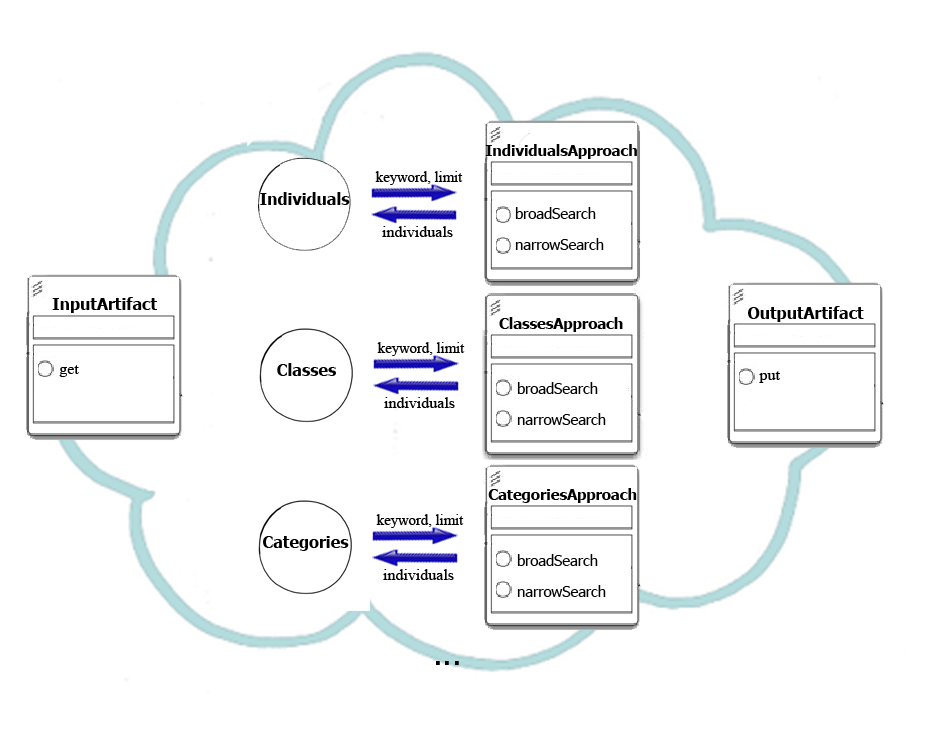
\includegraphics[width=.9\textwidth]{figura2icaart.png}
  \caption{Overview of the recommender model.}
  \label{fig:new2}
 \end{figure*}
 
As an example, the individual approach process the keywords in order to obtain individuals that contain the keyword in the properties db-prop:title or db-prop:name. A shorter version of the SPARQL query for the narrow search of this approach is shown below. The words preceded by the symbol @ are parameters that will be informed by the agents when calling the artifact's operation. The query states the prefixes, defines the result being returned at SELECT and the search criteria at WHERE. The filters ban the results that belong to categories which results are poor related with an educational context. The parameters that the agent informs in this query are the keyword being searched, the depth of the search, and the limit of results.

\begin{small}
\begin{verbatim}
PREFIX db-prop: <http://dbpedia.org/property/>
PREFIX dbpedia-owl:
   <http://dbpedia.org/ontology/>
PREFIX rdf:
   <http://www.w3.org/1999/02/22-rdf-syntax-ns#>
PREFIX rdfs:
   <http://www.w3.org/2000/01/rdf-schema#>
PREFIX dbpedia_cat:
   <http://dbpedia.org/resource/Category:>
PREFIX dcterms: <http://purl.org/dc/terms/>
PREFIX foaf: <http://xmlns.com/foaf/0.1/>
SELECT distinct ?object
WHERE {
{?object db-prop:title ?title . ?title
   <bif:contains> "+@keyword+" . }
UNION 
{?object  db-prop:name ?name. ?name
   <bif:contains> "+@keyword+" . }
filter (NOT EXISTS
   {?object dcterms:subject ?Category .
   ?Category skos:broader dbpedia_cat:Sports
   option(TRANSITIVE, T_DISTINCT,
   t_max(@t_max)) }) .
filter (NOT EXISTS
   {?object dcterms:subject ?Category .
   ?Category skos:broader dbpedia_cat:Companies
   option(TRANSITIVE, T_DISTINCT,
   t_max(@t_max)) }) .
}
LIMIT @limit
\end{verbatim}
\end{small}

Below we show a shorted version of the code for the classes\_approach agent. It starts by discovering the artifacts that it will use through the goal myTools. Those are the artifacts for input, output and the one specialized on the classes approach. Then the goal consumeItems checks if new keywords are available in the InputArtifact at 0.5 seconds intervals. When a keyword is obtained it is used in the processItem goal, which executes the semantic search. First, the agent calls the artifact's operation execute\_broad. the the agent uses the results from the broad search to execute a narrow search. If after executing the narrow search there are no results, the agent will send to the OutputArtifact the results from the broad search, otherwise the results from the narrow search will be sent. This decision is made by the goal decideOutcome. Before sending the results to the OutputArtifact through the put operation, the agent calls the operation execute\_getIndividuals to obtain the individuals from each class as the final result from the semantic search. 

\begin{small}
\begin{verbatim}
!observe.

+!observe : true 
  <- .wait(200); 
    ?myTools(A1, A2, Id);
    !consumeItems(Id).

+!consumeItems(Id): true
<- .wait(500);
get_for_ClassesApproach(Item);
!processItem(Item, Id);
!!consumeItems(Id).

(...)

+!processItem(Keyword, Id) : true
<-  execute_broad(Keyword, 30, R1)
   [artifact_id(Id)];
	execute_narrow(R1, R2)[artifact_id(Id)];
	isEmpty(R2, Test)[artifact_id("input")];
	!decideOutcome(R1, R2, Test, Id).	

+!decideOutcome(R1, R2, Test, Id) : Test
<- execute_getIndividuals(R1, 20, R3)
   [artifact_id(Id)];
	put(R3).
	
(...)
	
+?myTools(A1, A2, A3): true 
  <- lookupArtifact("input",A1);
  	 lookupArtifact("output",A2);
	 .my_name(N);
	 lookupArtifact(N,A3).
	 
(...)
\end{verbatim}
\end{small}

\section{Conclusion and Future Work}
\noindent In this paper we developed a recommender system where agents access the Semantic Web by means of artifacts that model the environment. The system is able to obtain recommendations for LO metadata using the partial knowledge provided by the user to process semantic queries on DBPedia through SPARQL. The contributions and results of this work can be observed in two points of view:

a) Metadata recommenders systems: To the best of our knowledge, in the context of recommenders specific for educational LO metadata there are no works available to compare our results with. The system developed in this paper is an initial prototype for this context. We noticed that our systems' recommendations were useful to obtain more information about a concept, but most of the time they were unrelated with the educational context. We believe that it happened because DBPedia isn't a semantic repository specific for educational purposes, then lacking the pedagogical information necessary for the recommendations.

b) Architectures that enable agents to access the Semantic Web: The main objective of our paper was to developed a model of system where agents can have access to the Semantic Web by means of artifacts, so this is context where we are able to make most of our comparisons. The main difference between our work and the related work (\cite{refB, refC, refA, refD, refE, refF}) regarding the access to the Semantic Web by agents is that in this work the integration is accomplished by means of artifacts.

Due to the adoption of artifacts, our model provides reusability: By using artifacts agents are able to access the Semantic Web without the need to implement code or an architecture specific for them. Also, conceptually any BDI agent is able to use artifacts are developed. Other relevant points are that artifacts decreases the computational burden on the agent side, since the agents just activate the desired operation at the artifact, and they can perform other tasks while the artifact process the operation.

The semantic artifacts use SPARQL queries with a predefined general structure. In the current version the customizable parts by the agents are the keywords being searched, the prefixes, the filters and some parameters of the search. In a future version we could use the functionality of internal properties of the artifacts, which can be modified at runtime by agents to change the services being offered by the artifact. So the agents would be able to customize the queries to DBPedia at runtime. Other possible future works include: real time recommendations; utilize the contents of the LO or the user's personal data as context; and an empirical evaluation of the system.

\bibliographystyle{sbc}
\bibliography{sbc-template}

\end{document}
